\section{Specific Requirements}
This section contains the detailed requirements for the Best Bike Paths (BBP) system. It provides a comprehensive description of the external interfaces, functional requirements, and non-functional constraints necessary for the development team to implement the solution.

\subsection{External Interface Requirements}
This subsection describes how the system interfaces with users, hardware, other software, and communications.

\subsubsection{User Interfaces}
The system is primarily accessed via a mobile application (Android/iOS). The user interface must be designed to be minimal and high-contrast to ensure legibility while cycling (Safety Critical).

\begin{itemize}
    \item \textbf{Map Visualization:} The UI shall display a map as the central element, rendering paths with color codes indicating their status (e.g., Green for ``Optimal'', Red for ``Poor'').
    \item \textbf{Controls:} Buttons for starting/stopping trips and reporting anomalies must be large and easily tappable to facilitate interaction during physical activity.
    \item \textbf{Notifications:} The system shall use non-intrusive notifications (audio cues or heads-up alerts) for automated detection alerts to minimize user distraction.
\end{itemize}

\subsubsection{Hardware Interfaces}
The mobile application interacts directly with the smartphone's hardware sensors to fulfill the automated data collection goals.

\begin{itemize}
    \item \textbf{GPS Receiver:} Used to track geolocation (latitude, longitude, altitude) and calculate real-time speed.
    \item \textbf{Accelerometer \& Gyroscope:} Used to detect vertical accelerations and device orientation changes indicative of road anomalies (e.g., potholes) or specific cycling movement patterns.
    \item \textbf{Local Storage:} The device's file system is used to buffer trip data and sensor logs temporarily when an internet connection is unavailable.
\end{itemize}

\subsubsection{Software Interfaces}
The BBP system interacts with the following external software entities:

\begin{itemize}
    \item \textbf{Map Service API} (e.g., Google Maps, OpenStreetMap): Used to retrieve map tiles and access the underlying road network topology.
    \item \textbf{Weather Service API:} Used to fetch meteorological data (Temperature, Wind Speed, Weather Condition) based on the specific timestamp and location coordinates of a trip.
    \item \textbf{Operating System} (Android/iOS): The app interfaces with the host OS to manage permissions (Location Always On, Background Processing) and utilize system notification services.
\end{itemize}

\subsubsection{Communication Interfaces}
\begin{itemize}
    \item \textbf{Protocol:} Communication between the Mobile Client and the Backend Server shall occur over HTTPS to ensure data confidentiality and integrity.
    \item \textbf{Data Format:} Data exchange (e.g., trip uploads, route requests) shall use JSON format over RESTful APIs.
\end{itemize}
%%%
\newpage
\subsection{Functional Requirements}

\subsubsection{Use case diagrams}
\begin{enumerate}
    \item \textbf{Unregistered User}
    \begin{figure}[H]
        \begin{center}
            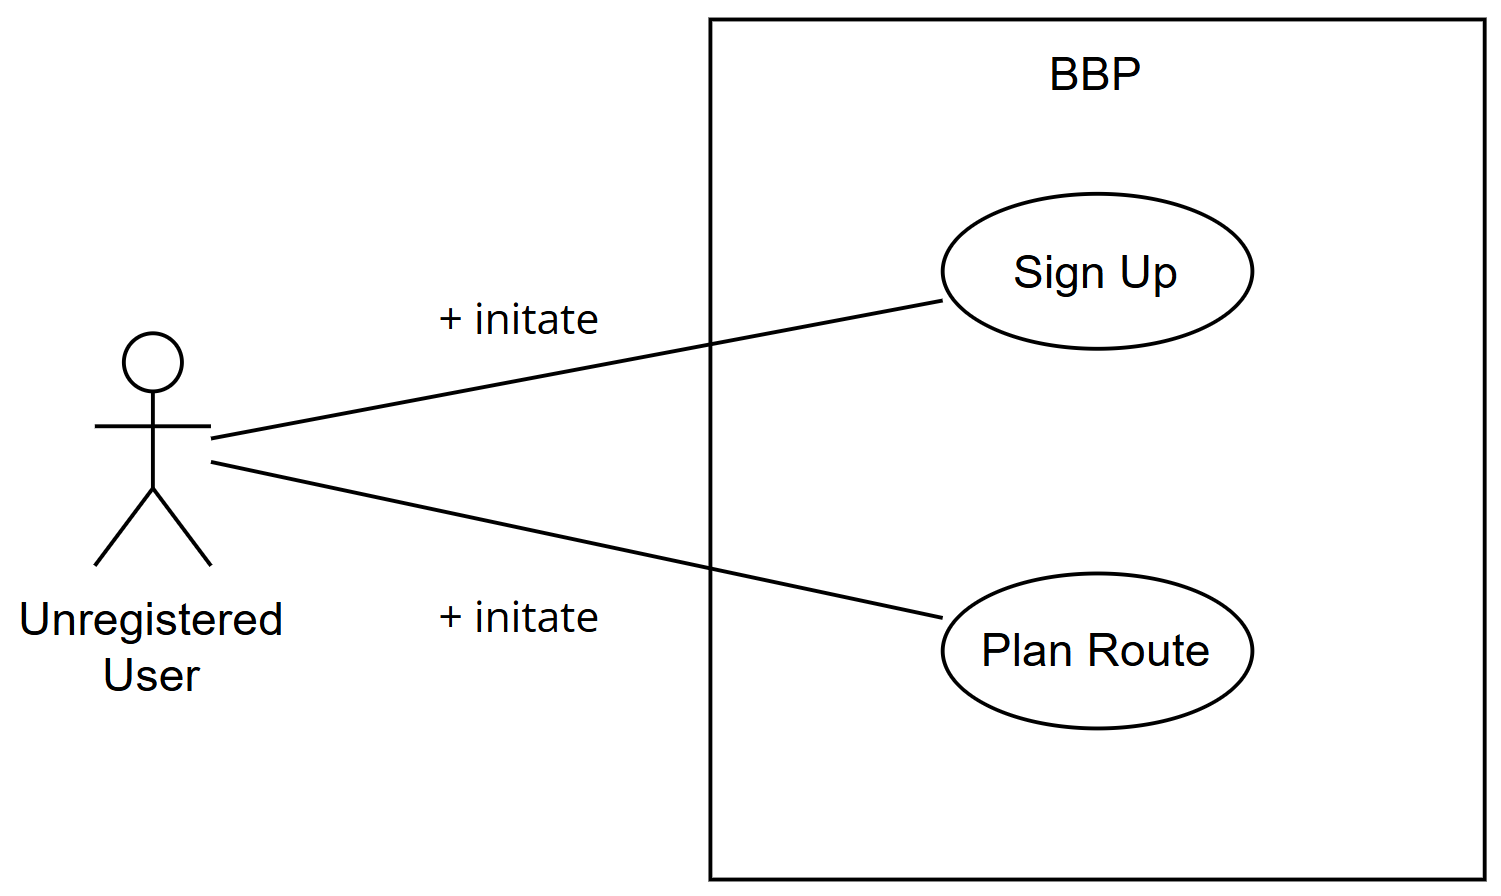
\includegraphics[width=0.8\textwidth]{RASD/img/section3/Unregistered_User.png}
            \caption{Unregistered User - Use Case Diagram}
        \end{center}
    \end{figure}
    \item \textbf{Registered User}
    \begin{figure}[H]
        \begin{center}
            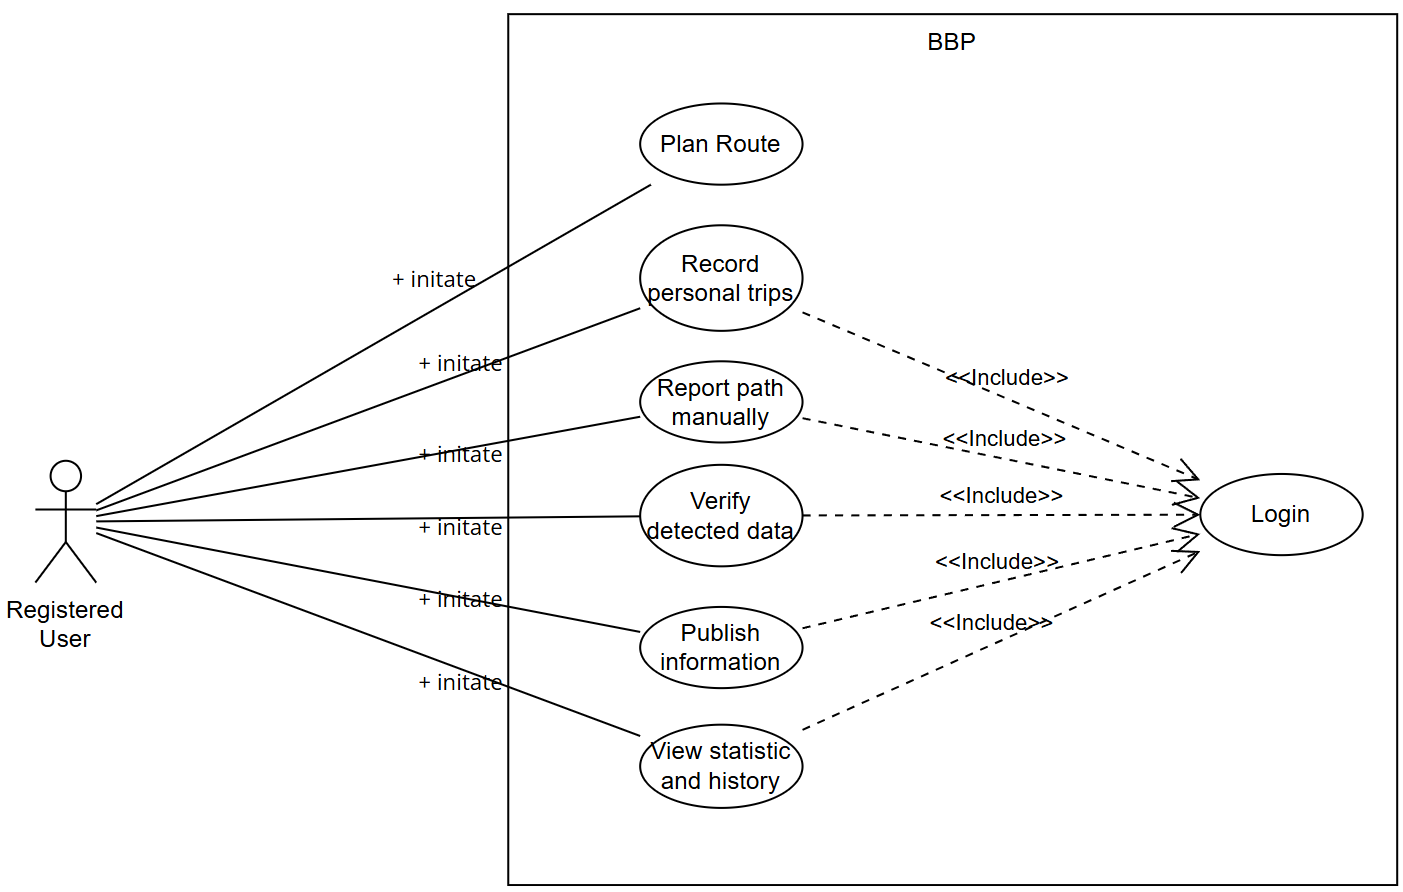
\includegraphics[width=\textwidth]{RASD/img/section3/Registered_User.png}
            \caption{Registered User - Use Case Diagram}
        \end{center}
    \end{figure}

\end{enumerate}

\subsubsection{Use Case Tables and Sequence Diagrams}



%%PLAN ROUTE
\begin{table}[H]
\centering
\begin{tabularx}{\textwidth}{|m{3.5cm}|X|}
\hline
\textbf{ID} & UC2 \\ \hline
\textbf{Name} & Plan Route \\ \hline
\textbf{Actor} & Unregistered User, Registered User \\ \hline
\textbf{Entry conditions} & The User has opened the application and accessed the ``Explore'' section. \\ \hline
\textbf{Input} & \texttt{origin}, \texttt{destination} \\ \hline
\textbf{Events flow} & 
    \begin{enumerate}[nosep, leftmargin=*, before=\vspace{0.3em}, after=\vspace{0.3em}]
        \item The application displays a map view with a search bar.
        \item The User enters the address for the ``Origin'' and ``Destination''.
        \item The User clicks the ``Find Route'' button.
        \item The System calculates available routes based on the Path Inventory and external map data.
        \item The application displays the map with the calculated routes drawn on it. The route with the highest score is highlighted in green.
        \item The application shows a summary card with details (distance, estimated time, and Path Score) for the best route.
        \item The User selects a specific route to view detailed segment information.
    \end{enumerate} 
    \\ \hline
\textbf{Exit conditions} & 
    \begin{itemize}[nosep, leftmargin=*, before=\vspace{0.3em}, after=\vspace{0.3em}]
        \item The optimal path is visualized on the user's screen.
        \item The User can proceed to navigation.
    \end{itemize}
    \\ \hline
\textbf{Output} & 
    \begin{itemize}[nosep, leftmargin=*, before=\vspace{0.3em}, after=\vspace{0.3em}]
        \item Map visualization of the routes.
        \item Route statistics (Path Score, Status, Distance).
    \end{itemize}
    \\ \hline
\textbf{Exceptions} & 
\textbf{No Path Found:} If no route connects the points, the application displays a generic error message ("No bike paths found") and keeps the User on the search view. \\ \hline
\end{tabularx}
\caption{Use Case 2: Plan Route}
\label{tab:uc2_planroute}
\end{table}
%% PLAN ROUTE SEQDIAG
\begin{figure}[H]
    \begin{center}
        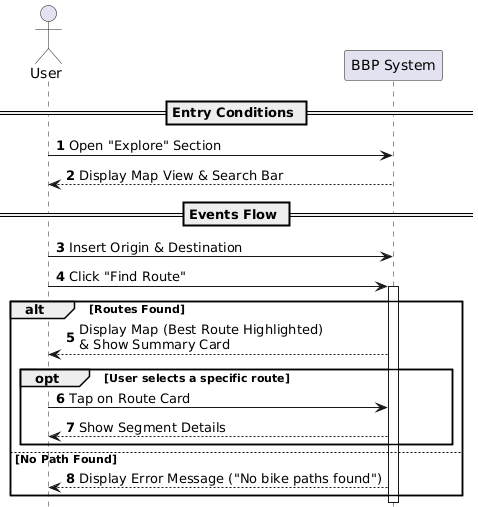
\includegraphics[width=\textwidth]{RASD/img/section3/SD2.png}
        \caption{Plan Route}
    \end{center}
\end{figure}
\newpage